\chapter{Expander Codes}
The main drawback of Reed-Solomon codes is the large alphabet size. Expander codes are codes that do not have this drawback.

It is a sparse graph with the property that the neighborhood of $S$ (small enough set) in the graph is larger than $S$ itself. To build an error-correcting code, it is best to start with a bipartite expander graph.
\section{Bipartite Expander Graphs}
\begin{definition}[$(\alpha,\beta)$-Bipartite Expander Graphs]
	A bipartite graph $G=(L,R,E)$ with bipartition $L,R$ is called an $(\alpha,\beta)$ expander, if for every set $S\subseteq L$ with $|S|\leq \alpha|L|$, the number of vertices in $R$ that are connected to $S$, i.e. $|\Gm(S)|\geq \beta|S|$
\end{definition}
We also introduce two notions which we will use wildly:
$$\Gm^{odd}(S)=\{j\in R\mid |\Gm(j)\cap S|=\text{odd}\}\quad \Gm^{+}(S)=\{j\in R\mid |\Gm(j)\cap S|=1\}$$
So $\Gm^{odd}(S)$ is the set of vertices of $R$ which have odd neighbors in $S$ and  $\Gm^{+}(S)$ is the set of unique neighbors of $S$
\begin{definition}[Unique Neighbor of $S$]
	Given $S\subseteq L$, the vertex $v\in R$ is  an unique neighbor of $S$ if $v$ is adjacent to exactly one vertex in $S$.
\end{definition}So we get $$\Gm^+(S)\subseteq \Gm^{odd}(S)\subseteq \Gm(S)$$
\begin{remark}
	For convenience we will take $G=(L,R,E)$ to be $(c,d)$ regular that is $G$ is left $c$ regular and right $d$ regular.
\end{remark}
\begin{definition}[$(\alpha,\beta)$-Unique Expander]
	$G=(L,R,E)$ is a $(\alpha,\beta)$-unique expander if $\forall\ S\subseteq L$ $$|S|\leq \alpha |L|\implies |\Gm^+(S)|\geq \beta |S|$$
\end{definition}
\begin{theorem}\label{uniqevertexexpander}
	If $G=(L,R,E)$ is $(\alpha,\beta)$-expander where $\beta>\frac{\alpha}{2}$ then it is a $(\alpha,2\beta -c)$-unique expander.
\end{theorem}
\begin{proof}
	Take $U=\gm^+(S)$ and $T=\Gm(S)\setminus \Gm^+(S)$. Now we know $$|U\cup T|=|\Gm(S)|\geq \beta |S|$$ We will count the number of edges between $S$ and $\Gm(S)$. Since $L$ is $c$ regular from left side total $c|S|$ edges are there. In right side for unique neighbors there are one edge for each unique neighbor and for other vertices there are at least $2$ edges.  So from right side at least $|U|+2|T|$ edges are there. So we have the relation $$|U|+2|T|\leq c|S|\implies |U|+2(|\Gm(S)-|U|)\leq c|S|\implies |U|\geq 2|\Gm(S)|-c|S|\geq (2\beta-c)|S|$$Since we are given that $\beta>\frac{c}2$ the graph is $(\alpha,2\beta-c)$-unique expander.
\end{proof}
\section{Expander Code}
We will take $|L|=n$ and $|R|=m$ from now on. And also by default we will assume $\beta> \frac{c}{2}$
\begin{definition}
	The $m\times n$ adjacency matrix $H$ of the $(\alpha,\beta)$-bipartite expander graph. Then $H$ is the parity check matrix of the corresponding expander code $C$. we denote the corresponding expander code of a $(\alpha,\beta)$-expander graph $G=(L,R,E)$ by $\mcC(G)$.
\end{definition}
\begin{remark}
	These codes are also called as \textit{Low Density Parity Check Codes}, because the parity check code $H$ is a sparse matrix. 
\end{remark}
\parinf
\textbf{Dimension:}  Since the parity check matrix is $m\times n$ matrix. The dimension of the code is $n-m=n-\frac{cn}{d}=n\lt(1-\frac{c}{d}\rt)$.

\textbf{Rate:} Rate of the code $1-\frac{c}{d}$.

\textbf{Distance:} The distance of the code is $\geq \alpha n$ (Proved below).\parinn

\begin{theorem}\label{distdeln}
	If $G=(L,R,E) $ is a $(\alpha,\beta)$-expander with $\beta>\frac{c}2$ then $$\delta(\mcC(G))\geq \alpha$$
	%\begin{tikzpicture}
%	\draw (0,0);
%\end{tikzpicture}
\end{theorem}
\begin{proof}
		Since the code is linear, it suffices to show that every codeword has hamming weight at least $\alpha n $. Assume the contrary.	Let $c=(c_1,\dots,c_n)\in \mcC(G)$ be a nonzero codeword of min weight. Suppose $wt(c)<\delta n$. Take $S=\{i\in L\mid c_i=1\}$. 
	
	Now by \thmref{uniqevertexexpander} $|\Gm^+(S)|\geq (2\beta-c)|S|>0$. So $\Gm^+(S)$ is nonempty. Every constraint in $\Gm^+(S)$ is a violated constraint. Hence contradiction \ctr. $wt(c)\geq \alpha n$.
\end{proof}
\begin{corollary}
	$G=(L,R,E)$ is $(c,d)$-regular  $(\delta,c(1-\eps))$-expander for some $\eps\in \lt(0,\frac12\rt)$ then $\delta(\mcC(G))>\delta$
\end{corollary}
From now on we will use the notion of $(\delta,c(1-\eps))$-expander.
\begin{theorem}
	$G=(L,R,E)$ is $(c,d)$-regular  $(\delta,c(1-\eps))$-expander for some $\eps\in \lt(0,\frac12\rt)$ then $$\delta(\mcC(G))>2\delta(1-\eps)$$
\end{theorem}
\begin{proof}
	Let $c$ is the min weight nonzero codeword. Take $S=\{i\in L\mid c_i=1\}$. From \thmref{distdeln} we have $|S|\geq \delta n$. Suppose $|S|<2\delta(1-\eps)n$ for contradiction. So we have $$\delta n\leq |S|< 2\delta(1-\eps)n$$ Fix any subset $T\subseteq S$ such that $|T|=\delta n$. Now 
	
	\begin{minipage}{0.40\textwidth}
		\begin{align*}
			|\Gm^{odd}(S)| & \geq |\Gm^+(S)|\\ & \geq |\Gm^+(T)|-|\Gm(S\setminus T)|\\ & \geq (c(1-2\eps)\delta n)-c|S\setminus T|\\ 
			& > (c(1-2\eps)\delta n)-c(\delta (1-2\eps))n=0
		\end{align*}
	\end{minipage}
	\hspace{2cm}
	\begin{minipage}{0.40\textwidth}
		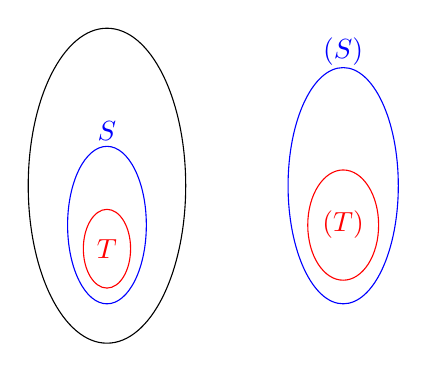
\begin{tikzpicture}
			\draw (0,0) ellipse (1cm and 2cm) ;
			\draw[blue] (0,-0.5) ellipse (0.5cm and 1cm) node[yshift=1.2cm] {$S$};
			\draw[red] (0,-0.8) ellipse (0.3cm and 0.5cm) node {$T$};
%			\draw[blue] (0,0.5) -- (3,1.5);
			\draw[blue] (3,0) ellipse (0.7cm and 1.5cm) node[yshift=1.7cm] {$\Gm(S)$} ;
			\draw[red] (3,-0.5) ellipse (0.45cm and 0.7cm) node {$\Gm(T)$};
		\end{tikzpicture}
	\end{minipage}
	\vspace{0.5cm}
	
	So $|\Gm^{odd}(S)|>0$. Hence there is a vertex $v\in R$ such that there is odd number of neighbors in $S$. Hence the constraint $v$ is not satisfied. Hence contradiction \ctr.
\end{proof}
\section{Decoding of Expander Codes}
\begin{algorithm}
\DontPrintSemicolon
\KwIn{$r=(r_1,\dots, r_n)$ with promise $\exs!\ c\in \mcC(G)$ such that $\delta(r,c)<\delta(1-2\eps)n$}
\Begin{
\tcp{{Step 1: (Initialization Phase)}}
$k\longleftarrow 0$\;
$x^{(k)}\longleftarrow r$\;
\ForEach{$j\in R$}{
\If{$\sum\limits_{i\in \Gm(j)}x_i=0$}{label $j$ as ``SAT"}
\Else{label $j$ as ``UNSAT"}
}
\ForEach{$i\in L$}{
$\mathsf{SAT}_i^{(k)}=\{j\in \Gm(i)\mid j\text{ labeled ``SAT"}\}$\;
$\mathsf{UNSAT}_i^{(k)}=\{j\in \Gm(i)\mid j\text{ labeled ``UNSAT"}\}$\;
}
\tcp{{Step 2:}}
\While{$\exs\ i\in L$  s.t. $|\mathsf{UNSAT}^{(k)}_i|>|\mathsf{SAT}^{(k)}_i|$}{
	$x_i^{(k+1)}\longleftarrow 1-x_i^{(k)}$\;
	$x_{i'}^{(k+1)}\longleftarrow x_{i}^{(k)}$ for all $i'\neq i$\;
	Update $\mathsf{SAT}_i^{(k)}$ and $\mathsf{UNSAT}_i^{(k)}$\;
	$k\longleftarrow k+1$\;
}
\tcp{{Step 3:}}
\Return $x^{k}$
}	
\caption{Linear Time Decoding Algorithm for Expander Code}
\end{algorithm}

\subsection{Analysis}
Let $r$ be the received word and $c\in \mcC(G)$ be the unique codeword such that $\delta(r,c)<\delta(1-2\eps)n$. Denote $$S^{(k)}=\{i\in L\mid x_i^{(k)}\neq c_i\}$$Hence we have $|S^{(0)}|<\delta(1-2\eps)n$. Also we will use the set $\mathsf{UNSAT}^{(k)}$ to denote the set of unsatisfied right constraints at $k$th step. Similarly for $\mathsf{SAT}^{(k)}$.
\begin{lemma}\label{exdecodelem1}
	If $\eps\in\lt( 0,\frac14\rt)$ and $0<|S^{(k)}|\leq \delta n$ then $\exs\ i\in L$ such that $|\mathsf{UNSAT}_i|>|\mathsf{SAT}_i|$.
\end{lemma}
\begin{proof}
	First notice that all unique neighbors of $S^{(k)}$ are unsatisfied at $k$th iteration. $\eps\in \lt(0,\frac14\rt)$ hence the graph is $(\delta,c(1-\eps))$-expander it is  $(\delta,c(1-2\eps))$-unique expander by \thmref{uniqevertexexpander}. Hence $$|\mathsf{UNSAT}^{(k)}|\geq c(1-2\eps)|S^{(k)}|> \frac{c}{2}|S^{(k)}|$$Hence, $\exs\ i\in S^{(k)}$ such that $|\mathsf{UNSAT}_i^{(k)}|>\frac{c}2$. Now the degree of $i$ is c. Hence $|\mathsf{UNSAT}_i^{(k)}|>|\mathsf{SAT}_i^{(k)}|$. 
\end{proof}
Since for each iteration the distance between $x^{(k)}$ and $c$ is at most $\delta n$, $c$ is the only codeword which is nearest to $x^{(k)}$. Hence the nearest codeword for each iteration stays the same.

Now in the algorithm there are two things to observe.
\begin{observation}
	The number of unsatisfied right constraints is always decreasing.
\end{observation}
\begin{observation}
	$|S^{(k)}-S^{(k+1)}|=1$
\end{observation}
\begin{lemma}\label{exdecodelem2}
	$|S^{(0)}|<\delta(1-2\eps)n\implies |S^{(k)}|<\delta n$.
\end{lemma}
\begin{proof}
	Initially $\mathsf{UNSAT}^{(0)}\subseteq {\Gm(S^{(0)})}$ since the unsatisfied constraints are the subset of the neighbors of errors. Hence $$|\mathsf{UNSAT}^{(0)}|\leq|{\Gm(S^{(0)})}|\leq c|S^{(0)}|<c|S^{(o)}|<c\delta(1-2\eps)n$$
	
	Suppose there exists a $k'$ such that $|S^{(k')}|\geq \delta n$. By the observation there exists $k$ such that $|S^{(k)}|=\delta n$. Hence $$|\mathsf{UNSAT}^{(k)}|>|\Gm^+(S^{(k)})|\geq \delta n\cdot c(1-2\eps)$$But the $|\mathsf{UNSAT}^{(k)}|$ keeps decreasing so it can not start with less than $c\delta(1-2\eps)n$ and at some point is $\geq \delta n\cdot c(1-2\eps)$. Hence contradiction \ctr.
\end{proof}

At $k$th iteration  suppose the  number of unsatisfied constraints is nonzero and $|S^{(k)}|<\delta n$. Since number of  unsatisfied constraints is nonzero $|S^{(k)}|> 0$. By \lmref{exdecodelem1}  there exists an $i\in L$ such that $|\mathsf{UNSAT}_i|>|\mathsf{SAT}_i|$. Hence the algorithm will find some vertex which has more unsatisfied constraints than satisfied constraints and flip its bit and proceed to the next iteration. With this process the number of unsatisfied constraints reduced by at least 1. Thus the algorithm will keep reducing the number of unsatisfied constraints till it becomes zero because if its not zero at any $j$th iteration and then $|S^{(j)}|>0$ and hence by the above argument it will proceed. Once the  number of unsatisfied constraints becomes zero cause then the final output, suppose $x$ satisfies all the right constraints. Hence it is indeed a codeword and since the nearest codeword at each iteration stays the same $x=c$. 
\subsection{Time Complexity}
\begin{enumerate}
	\item Preprocessing Stage: For each $j\in R$ to check $\sum\limits_{i\in \Gm(j)}x_i=0$ it takes $O(d)$ time. Hence the first for loop takes $O(md)$ time. Now for each vertex in $L$ we keep the number of unsatisfied constraints which are neighbor of that vertex. We also keep a list of vertices in $L$ which have more unsatisfied constraints than satisfied constraints. This can be done in $O(cn)$ time.
	\item In each iteration of the while loop instead of searching for a vertex with more unsatisfied constraints than satisfied constraints we remove an element of $Q$. \parinn
	
	After flipping the vertex we update the list of unsatisfied constraints in $R$ in $O(c)$ time. Then we  will update the number of unsatisfied constraints associated with each element of in $L$ which are neighbors of the neighbors of $i$ i.e. the vertices in  $\Gm(\Gm(i))$ in $O(cd)$ time. Since after the bit flip the previously unsatisfied constraints are satisfied in $\Gm(i)$ and the previously satisfied constraints are now unsatisfied. For each vertex $j\in\Gm(i)$ if $j$ was previously unsatisfied then we will subtract 1 from the number of unsatisfied constrains of the neighbors of $j$ and if $j$ was previously satisfied then we will add 1 for any previously satisfied constraint to the number of unsatisfied constrains of the neighbors of $j$. Now from $Q$ we will remove the elements which have lesser unsatisfied constraints than satisfied constraints and add the.
	
	After updating the number of unsatisfied constraints of each vertex in $\Gm(\Gm(i))$ we will add the vertices which have more unsatisfied constraints than satisfied constraints into $Q$ and remove the vertices which have lesser unsatisfied constrains than satisfied constraints. This all can be done in $O(cd)$ time since $|\Gm(\Gm(i))|\leq cd$. Since $c,d$ are constants every thing inside each iteration can be done in constant time.
	\item In each iteration the number of unsatisfied constraints reduces by at least 1. The original number of unsatisfied constraints is at most $c\delta (1-2\eps)n$. (\thmref{exdecodelem2}). Then the total number of iterations is at most $c\delta(1-2\eps)n=O(n)$.
\end{enumerate}
Hence the algorithm decodes the received word in $O(n)$ time.